\documentclass[10pt,a4paper]{article}

\usepackage{fancyvrb}
\usepackage{caption}
\usepackage{float}
\usepackage{graphicx}
\usepackage{csquotes}

\begin{document}
\author{Supervisor: Atze Dijkstra\\\\Rick Klomp\\Student number: 5540232}
\title{Experimentation project\\Functional Programming in Spreadsheets}
\maketitle
\pagebreak

\section{Introduction}
Popular spreadsheet programs (e.g. Excel, LibreOffice) provide a
domain specific language to manipulate data. These DSLs are Turing complete (Hermans, 2013). Thus,
they're in principal as powerful as any other programming language.
However, many features known from languages such as Haskell are not provided by these languages.
Examples of these features include (but are not limited to):
\begin{itemize}
\item Higher order functions
\item Lazy evaluation
\item List comprehension
\end{itemize}
This has raised the question if the experience of spreadsheet programming can be improved by
providing a cleanly designed language that provides powerful mechanisms known from functional
programming languages.
\\\\
To initiate research in the area, this project has been performed to define an API that provides
an interface for spreadsheet computations as well as to experiment with a basic application of
the API. Results and findings of these topics are discussed in sections \ref{API} and
\ref{API application} respectively. Section \ref{Prior work} presents some related prior research
that has been performed.

\section{Prior work}
\label{Prior work}
There has been some research performed on the subject before.
\\\\
Haxcel has resulted from a MSc thesis project:
\begin{displayquote}[Lisper, 2005]
Haxcel is a spreadsheet-like interface to Haskell, where declerations can be edited and values of
different variables monitord as declarations are updated.
\end{displayquote}
Unfortunately, this project doesn't seem to have been succeeded.
\\\\
Furthermore, Wakeling has performed research on embedding functional languages such as Haskell
inside a standard spreadsheet such as Excel (Wakeling, 2007).

\section{API}
\label{API}
The API abstracts over four layers of spreadsheet computation functionality.
Each layer is covered by one of the following type classes:
\begin{itemize}
\item Spreadsheet
\item Cell
\item Expr
\item Var
\end{itemize}
These abstraction layers are further discussed in sections \ref{Spreadsheet abstraction} through
\ref{Var abstraction} respectively. Furthermore, section \ref{Annotated text} discusses a feature
considering visually highlighting references that is present in popular spreadsheet programs,
but is probably not implementable in a sensible way using the current API.

\subsection{Spreadsheet abstraction}
\label{Spreadsheet abstraction}
\begin{minipage}{\linewidth}
\begin{Verbatim}[numbers=left,stepnumber=1,numbersep=5pt]
class (MonadState s m, Var v, Expr e v rm, Cell c e v) =>
          Spreadsheet s c e v m rm | s -> c, s -> v, s -> m where
  updateEvals :: m ()
  getCell     :: Pos -> m (Maybe c)
  setCell     :: Pos -> c -> m ()
\end{Verbatim}
\captionof{figure}{The Spreadsheet type class.}\label{Spreadsheet type class}
\end{minipage}
\\\\
The definition of the Spreadsheet type class is given in figure \ref{Spreadsheet type class}.
This layer functions as an encapsulation over the grid of Cells. The updateEvals function
defines the interface for initiating a complete spreadsheet evaluation.
With getCell and setCell it provides a way to access the next layer of abstraction (i.e. the
Cell abstraction, see section \ref{Cell abstraction}). All functions depend on the state of the
spreadsheet, thus they're run in a MonadState environment.

\subsection{Cell abstraction}
\label{Cell abstraction}
\begin{minipage}{\linewidth}
\begin{Verbatim}[numbers=left,stepnumber=1,numbersep=5pt]
class (MonadReader (Map v e) m, Var v, Expr e v) =>
          Cell c e v m | c -> e, c -> v, v -> m, e -> m where
  evalCell      :: c -> m c
  parseCell     :: c -> c
  getEval       :: c -> Maybe e
  getText       :: c -> String
\end{Verbatim}
\captionof{figure}{The Cell type class.}\label{Cell type class}
\end{minipage}
\\\\
Figure \ref{Cell type class} gives the definition of the Cell type class.
The Cell abstraction enforces a state machine-like usage. Prior to calling evalCell, the Cell's
content should succesfully have been parsed by the parseCell function. Any definitions of
global variables that the cell's expression requires during evaluation should be supplied through
the MonadReader environment. Similarly, prior to calling getEval, the Cell's expression should
succesfully have been evaluated by the evalCell function. These functions don't return information
showing if something failed, thus the state should somehow be stored and manipulated inside the
Cell datatype (:: c). It might be useful to refine the types of these functions to reflect the
state behaviour as well.

\subsection{Expr abstraction}
\label{Expr abstraction}
\begin{minipage}{\linewidth}
\begin{Verbatim}[numbers=left,stepnumber=1,numbersep=5pt]
class (MonadReader (Map v e) m, Var v) =>
          Expr e v m | e -> v, v -> m, e -> m where
  evalExpr        :: e -> m e
\end{Verbatim}
\captionof{figure}{The Expr type class.}\label{Expr type class}
\end{minipage}
\\\\
In figure \ref{Expr type class} the definition of the Expr type class is given. This layer
of abstraction defines an interface to the spreadsheet language. All global variables that are
required for evaluating an expression should be supplied through the MonadReader instance.
It might be useful to refine the types of this function to reflect the state behaviour as well.

\subsection{Var abstraction}
\label{Var abstraction}
\begin{minipage}{\linewidth}
\begin{Verbatim}[numbers=left,stepnumber=1,numbersep=5pt]
class Var v where
\end{Verbatim}
\captionof{figure}{The Var type class.}\label{Var type class}
\end{minipage}
\\\\
Figure \ref{Var type class} gives the definition of the Var type class.
This layer is currently purely used to allow for different kind of variable encodings within
languages. Perhaps this part of the API should be extended with functions once some kind of
annotated text mechanism has been added (see section \ref{Annotated text}).¬

\subsection{Annotated text}
\label{Annotated text}
\begin{figure}[H]
\centering
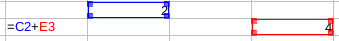
\includegraphics[width=0.75\textwidth]{referenceHighlighting.png}
\caption{Visual highlighting of references in LibreOffice.}
\label{Visual highlighting references}
\end{figure}
Currently, the API probably doesn't provide enough flexibility at some places to allow for adding
features in a sensible way such as visually highlighting references (see figure \ref{Visual highlighting references}).
Information stored at the higher layers of the API (e.g. the state of the spreadsheet) isn't
by default available at lower layers of the API (e.g. in the evalExpr function).
It would most likely be wise to change the API in such a way that all information is provided
through a single MonadState instance, and that all functions of the API run in this monadic
environment.

\section{API application}
\label{API application}
A basic spreadsheet program has been developed to experiment with the API.
Section \ref{Experimentation API application} discusses implementation specifics of this
spreadsheet program.
\\\\
The API abstracts over the backend matters that stay constant regardless of the implementation.
It seems that some of the frontend matters can be abstracted over as well. In section
\ref{Frontend abstraction} a mechanism is discussed that can probably be abstracted over.
\\\\
There are arguably issues with popular spreadsheet programs considering other areas than the
expresssions language. These are briefly discussed in section \ref{Spreadsheet miscellaneous issues}.

\subsection{Experimentation API application}
\label{Experimentation API application}
The expression language that is provided is Lambda calculus extended with three small features:
\begin{itemize}
\item Back and forth computation between Church numerals and Haskell numeral notation. The predefined
function toInt translates a Church numeral to a Haskell numeral, and Haskell numerals are translated to
Church numerals during parsetime
\item Back and forth computation between Church lists and Haskell list notation. The predefined
function toInt translates a Church list to a Haskell list, and Haskell lists are translated to Church
lists during parsetime
\item Cell reference variables (e.g. 1A, 5B)
\end{itemize}
All technical challenges have been solved in naive ways.
For example, when a cell expression has been modified, the entire sheet is recomputed. If during
this recomputation an evaluation differs from a prior evaluation, the change is pushed and the entire
process is repeated (i.e. the entire sheet is again recomputed).

\subsection{Frontend abstraction}
\label{Frontend abstraction}
All popular spreadsheet programs seem to have atleast two modes a user can be in,
where one mode is for moving items (e.g. the cursor, cells) through the spreadsheet and the other
is for editing items (e.g. cell content, figures).
If it is indeed the case that for any possible spreadsheet program atleast two user modes are
provided it is probably useful to abstract (some of) the mode changing behaviour to higher level
mechanisms.

\subsection{Spreadsheet miscellaneous issues}
\label{Spreadsheet miscellaneous issues}
Dan Halbert seems to have a valid remark to current popular spreadsheet programs:
\begin{displayquote}[Halbert, 2012]
I think hidden formulas is one of the big issues with spreadsheets. [...] The other big problem
is the awkardness of assigning meaningful names to cells and blocks of cells.
\end{displayquote}
A solution for both of these issues might be to add a secondary environment to the spreadsheet program
wherein regular code can be written. For example, toplevel definitions could behave like global
variables, and can subsequently be referenced to in cell expressions.

\clearpage
\section{Conclusion}
An API has been defined that provides an abstraction over spreadsheet computation functionality.
It most likely needs to be refined to allow some spreadsheet features to be defined in
sensible ways.
\\\\
Furthermore, the problem area in general has been researched. There has been some prior research
performed. However, no extensive research has been performed, which in this case is probably
needed in order to get a clear picture of the benefits and cost of functional programming spreadsheets.

\section*{Bibliography}
Halbert, D. (2012, November). \textit{Let's fix spreadsheets}.

Retrieved from http://www.lambda-the-ultimate.org/node/4626
\\\\
Hermans, F. (2013, September). Excel Turing Machine [Web log post].

Retrieved from http://www.felienne.com/archives/2974
\\\\
Wakeling, D. (2007). Spreadsheet functional programming.

Journal of Functional Programming, 17, pp 131-143

\end{document}
